\documentclass{book}
\usepackage[utf8]{inputenc}
\usepackage[russian]{babel}
\usepackage{color}
\usepackage{hyperref}
\usepackage{amsfonts}
\usepackage{graphicx}
\hypersetup{
	colorlinks=true,
	linkcolor=blue,
   	linktoc=all
}

\begin{document}
\tableofcontents

\pagestyle{plain}

\addcontentsline{toc}{chapter}{Занятие 1. Элементы комбинаторики}
\chapter*{Занятие 1. Элементы комбинаторики}

\addcontentsline{toc}{section}{Контрольные вопросы и задания}
\section*{Контрольные вопросы и задания}

\subsubsection*{Сформулируйте основной принцип комбинаторики (правило умножения).}

Если множества $A_1, ..., A_m$ содержат соответственно $n_1, ..., n_m$ элементов, то количество m-мерных векторов, которые получают выбором по одному элементу из каждого множества равно $n_1\cdot n_2\cdot...\cdot n_m$.

\subsubsection*{Что называется сочетанием из n элементов по k?}

В комбинаторике сочетанием из n по k называется набор k элементов, выбранных из данного множества, содержащего n различных элементов.

\subsubsection*{Чему равно число сочетаний из n элементов по k?}

Если некоторое множество содержит n элементов, то количество её k-элементных подмножеств равно $$C_n^k=C_n^{n-k}=\frac{n!}{k!\left(n-k\right)!=\frac{n\cdot\left(n-1\right)\cdot...\cdot\left(n-k+1\right)}{k!}},$$ где $n!=1\cdot 2\cdot...\cdot n$. Считается, что $0!=1$.

\subsubsection*{Что называется сочетанием с повторениями из n элементов по k?}

Сочетанием (комбинацией) с повторениями называется набор из n элементов, каждый из которых может быть одного из k типов.

\subsubsection*{Чему равно число сочетаний с повторениями из n элементов по k?}

Количество разных комбинаций из элементов n типов по k с повторениями равно $$C_n^k=C_{n+m-1}^{m-1}=C_{n+m-1}^n.$$

\subsubsection*{Что называется размещением из n элементов по k?}

Размещения из n элементов по k --- это упорядоченные k-элементные подмножества множества, которое состоит из n элементов.

\subsubsection*{Чему равно число размещений из n элементов по k?}

Количество размещений из n элементов по k равно $$A_n^k=k!C_n^k=n\cdot(n-1)\cdot...\cdot(n-k+1).$$

\subsubsection*{Чему равно число перестановок множества из n элементов?}

Количество перестановок равно $n!$.

\subsubsection*{Чему равно число способов разбиения множества из n элементов на m непересекающихся неупорядоченных подмножеств, которые содержат соответственно $k_1, ..., k_m$ элементов?}

Первое подмножество содержит $k_1$ элемент. Количество комбинаций, которыми можно выбрать эти элементы, равно $C_n^{k_1}$. Второе подмножество содержит $k_2$ элементов, тогда его элементы можно выбрать $C_{n-k_1}^{k_2}$ способами. Подмножество под номером m содержит $k_m$ элементов. Эти элементы можно выбрать из оставшихся $\left(n-k_1-k_2-...-k_{m-1}\right)$ $C_{n-k_1-k_2-...-k_{m-1}}^{k_m}$ способами. Число способов разбиения множества из n элементов на m непересекающихся неупорядоченных подмножеств равно $$C_n^{k_1}\cdot C_{n-k_1}^{k_2}\cdot...\cdot C_{n-k_1-k_2-...-k_{m-1}}^{k_m}=\prod\limits_{i=1}^mC_{n-\sum\limits_{j=0}^{i-1}k_j}^{k_i}.$$ Так как $$n=k_1+k_2+...+k_m=\sum\limits_{i=1}^m k_i=K_i,$$ то произведение можно записать в виде $$\prod\limits_{i=1}^mC_{K_i}^{k_i}.$$

\addcontentsline{toc}{section}{Домашние задачи}
\section*{Домашние задачи}

\subsubsection*{1.16.}

\textit{Задание.} Подсчитать, сколько трёхзначных чисел можно записать с помощью: а) цифр 0, 1, 2, 3, 4, 5; б) цифр 0, 1, 2, 3, 4, 5, если каждую из цифр использовать не больше одного раза.

\textit{Решение.} Трёхзначное число можно рассматривать как трёхмерный вектор. Первой компонентой этого вектора может быть любая цифра из множества $$A_1={1, 2, 3, 4, 5}$$ (запись числа не может начинаться с 0).

а) На остальных позициях может стоять любая цифра, то есть $$A_i={0, 1, 2, 3, 4, 5}, i=2, 3.$$ Отсюда имеем, что из указанных цифр можно составить $5\cdot 6\cdot 6=180$ трёхзначных чисел.

б) На остальных позициях могут стоять любые цифры (кроме тех, что стояли на предыдущих позициях). Отсюда имеем, что из указанных цифр можно составить $5\cdot 5\cdot 4=100$ трёхзначных чисел.

\subsubsection*{1.17.}

\textit{Задание.} Подсчитать количество пятизначных чисел, которые делятся на 5.

\textit{Решение.} Пятизначное число можно рассматривать как пятимерный вектор. Первой компонентой этого вектора может быть любая цифра из множества $$A_1={1, 2, 3, 4, 5, 6, 7, 8, 9}$$ (запись числа не может начинаться с 0), а на остальных позициях (кроме последней) может стоять любая цифра, то есть $$A_i={0, 1, 2, 3, 4, 5, 6, 7, 8, 9}, i=2, 3, 4.$$ На последней позиции может стоять цифра из множества $A_5={0, 5}$ (чтобы число делилось на 5, оно должно оканчиваться на 0 или 5). Отсюда имеем, что можно составить $9\cdot 10\cdot 10\cdot 10\cdot 2=18000$ пятизначных чисел, которые делятся на 5.

\subsubsection*{1.18.}

\textit{Задание.} Замок компьютерного центра состоит из пяти кнопок, пронумерованных от 1 до 5. Чтобы открыть замок, необходимо первые две определённые кнопки нажать одновременно, а потом одну за другой нажать другие три кнопки в определённой последовательности. Подсчитать количество способов закодировать вход в компьютерный центр.

\textit{Решение.} Рассмотрим 3 случая: 

а) сначала необходимо нажать две разные кнопки, далее их отпускают, и все остальные кнопки могут быть любыми; 

б) первые две кнопки держатся нажатыми, следующие кнопки не могут быть такими, как первые две; 

в) нельзя нажать одну и ту же кнопку больше одного раза (кнопки остаются нажатыми).

Количество способов нажать первые две кнопки равна количеству двухэлементных подмножеств в множестве из пяти элементов, то есть $$C_5^2=\frac{5!}{2!\left(5-2\right)!}=10.$$

В случае а) количество способов закодировать вход в компьютерный центр равно $$C_5^2\cdot 5^3=1250.$$ Общая формула: $C_N^n\cdot N^m$, где N --- количество кнопок, n кнопок нажимаются вместе, а затем m кнопок --- по очереди.

В случае б) после нажатия двух кнопок, остаётся только 3 кнопки, которые необходимо нажать в правильном порядке, поэтому количество способов по предыдущей формуле равно $$C_5^2\cdot 3^3=270.$$

В случае в) все кнопки должны быть нажаты один раз, поэтому количество способов закодировать вход равно $$C_5^2\cdot 3\cdot 2\cdot 1=60.$$

\subsubsection*{1.19.}

\textit{Задание.} Колоду игральных карт (52 карты, 4 масти по 13 карт в каждой) тщательно перетасовали. Подсчитать количество способов выбрать из неё 6 карт без возвращения так, чтобы среди них: а) был пиковый король; б) были представители всех мастей; в) было ровно 5 карт одной масти.

\textit{Решение.}

а) Выбрать пикового короля есть только один способ. Остальные 6 карт могут быть любыми из оставшихся 51 карты. Выбрать эти 5 карт можно $C_{51}^5$ способами. Отсюда имеем, что из колоды можно выбрать 6 карт, среди которых был бы пиковый король, $1\cdot C_{51}^5$ числом способов.

б) Сначала выберем по одной карте каждой масти. Количество способов выбрать одну карту определённой масти равно $C_{13}^1$, так как имеется 13 карт каждой масти. Так как всего есть 4 масти, то нужно выбрать 4 карты (по одной карте каждой масти). Тогда количество способов выбрать 4 карты разных мастей равно $$C_{13}^1\cdot C_{13}^1\cdot C_{13}^1\cdot C_{13}^1=\left(C_{13}^1\right)^4.$$ Остаётся выбрать две произвольные карты из оставшихся. После выбора четырёх карт разных мастей в колоде осталось $52-4=48$ карт. Число способов выбрать из них две карты равно $C_{48}^2$. Отсюда имеем, что количество способов выбрать из данной колоды 6 карт без возвращения таким образом, чтобы среди них были представители всех мастей, равно $$\left(C_{13}^1\right)\cdot C_{48}^2.$$

в) Сначала нужно выбрать 5 карт одной масти. В одной масти 13 карт, следовательно число способов выбрать 5 карт одной масти равно $C_{13}^5$. Так как всего мастей 4, и нам не важно, какой именно масти будут 5 вытянутых карт (главное, чтобы одной), то число способов будет равно $$4\cdot C_{13}^5.$$ Шестая карта должна быть любой, но отличатся с предыдущими пятью мастью, то есть её можно выбрать из $52-13=39$ карт. Число способов это сделать равно $C_{39}^1$. Отсюда имеем, что число способов выбрать из колоды карт 6 карт так, чтобы среди них было ровно 5 карт одной масти, равно $$4\cdot C_{13}^5\cdot C_{39}^1.$$

\subsubsection*{1.20.}

\textit{Задание.} Сколькими способами можно разместить 10 одинаковых открыток в 4 почтовых ящиках так, чтобы: а) не было пустых ящиков; б) во втором ящике было 3 открытки.

\textit{Решение.} Будем рассматривать несколько открыток как одно целое и раскладывать как одну большую открытку. Можем посчитать количество возможных разложений m склеенных открыток так же, как и одной обычной. Теперь мы говорим, что в ящике может находиться только одна открытка, либо обычная, либо большая, состоящая из нескольких открыток.

а) Рассмотрим случай, когда в каждый ящик должна быть помещена хотя бы одна открытка. Используем метод перегородок. Выложим открытки в ряд. Для определения расклада открыток по четырём почтовым ящикам разделим ряд тремя перегородками на 4 группы: первая группа для первого ящика, вторая --- для второго и так далее. Таким образом, число вариантов раскладки открыток по ящикам равно числу способов разложения трёх перегородок. Перегородки могут стоять на любом из 9 мест (между 10 открытками --- 9 промежутков). Поэтому число возможных расположений равно $C_9^3$.

б) Рассмотрим случай, когда во второй ящик должны быть помещены 3 открытки. Поскольку открытки одинаковые, то во второй ящик можно сразу положить 3 открытки. В этом случае нужно распределить $10-3=7$ одинаковых открыток между тремя почтовыми ящиками.

Используем метод перегородок. Рассмотрим ряд из 9 предметов: 7 одинаковых открыток и 2 одинаковые перегородки, расположенных в произвольном порядке. Каждый такой ряд однозначно соответствует некоторому способу раскладки открыток по ящикам: в первый ящик попадают открытки, расположенные левее первой перегородки, во второй --- расположенные между первой и второй перегородками и т.д. (между какими-то перегородками открыток может и не быть). Поэтому число способов раскладки открыток по ящикам равно числу различных рядов из 7 открыток и 2 перегородок, т.е равно $C_9^2$ (ряд определяется теми двумя местами из 9, на которых стоят перегородки).

\subsubsection*{1.21.}

\textit{Задание.} Сколькими способами можно распределить 10 путёвок среди 10 студентов (по одной каждому), если: а) все путёвки разные; б) есть 4 путёвки одного типа и 6 --- другого?

\textit{Решение.}

а) Количество возможных перестановок 10 разных путёвок равно $10!$.

б) Если будем считать все 10 элементов перестановки с повторениями различными, то всего различных вариантов перестановок 10 путёвок --- $$(4+6)!=10!.$$ Однако среди этих перестановок не все различны. Все путёвки одного типа можно переставлять местами друг с другом, и от этого перестановка не изменится. Точно так же, можем переставлять путёвки другого типа. Таким образом, перестановка может быть записана $4!6!$ способами. Следовательно, число различных перестановок с повторениями равно $$\frac{(4+6)!}{4!6!}=\frac{10!}{4!6!}.$$

\subsubsection*{1.22.}

\textit{Задание.} Доказать, что количество неубывающих путей на r-мерной целочисленной решётке $$\mathbb{Z}_+^r={\left(i_1, ..., i_r\right): i_1, ..., i_r=0, 1, 2, ...},$$ которые начинаются в точке $\left(0, ..., 0\right)$ и приводят в точку $\left(n_1, ..., n_r\right)$, равно $$C_N\left(n_1, ..., n_r\right)=\frac{N!}{n_1!...n_r!},$$ где $N=\sum\limits_{i=1}^rn_i$. (Путь считается неубывающим, если на каждом шаге изменяется только одна координата, увеличиваясь на единицу.)

\subsubsection*{1.23.}

\textit{Задание.} Из 100 студентов английский язык знают 28, немецкий --- 30, французский --- 42, английский и немецкий --- 8, английский и французский --- 10, немецкий и французский --- 5, а все три языка знают 3 студента. Сколько студентов не знают ни одного языка?

\textit{Решение.} Условие задачи представлено на рисунке \ref{fig:123} в виде диаграммы Эйлера-Венна. 

\begin{figure}[h!]
  \centering
  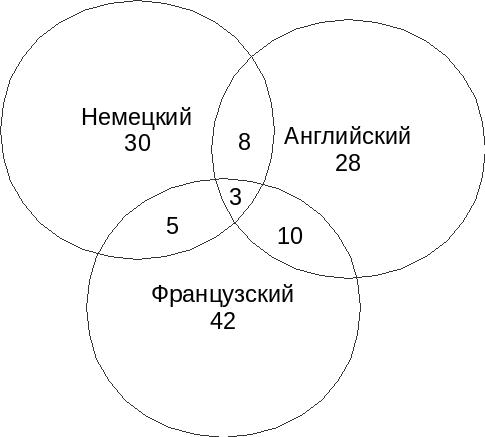
\includegraphics[width=.4\textwidth]{./pictures/1_23.png}
  \caption{Диаграмма Эйлера-Венна для задачи 1.23}
  \label{fig:123}
\end{figure}

Сначала найдём, сколько студентов знает хотя бы один язык. Это есть мощность (количество элементов) объединения трёх множеств: Английский, Немецкий и Французский, которые обозначим первыми буквами. Мощность объединения трёх множеств можно найти как сумму мощностей этих множеств, но, так как они пересекаются, необходимо отнять мощности их пересечений и добавить пересечение всех трёх множеств, потому что его отняли дважды. Имеем $$|H\bigcup A\bigcup\Phi|=|H|+|A|+|\Phi|-|H\bigcap A|-|A\bigcap\Phi|-|H\bigcap\Phi|+|H\bigcap A\bigcap\Phi|=$$$$=30+42+28-5-8-10+3=80.$$

Все остальные студенты из ста не знают ни одного языка. Их $100-80=20$.

\end{document}
